\section[\textlatin{Null}] {\textgreek {Ελλιπείς τιμές}, \textlatin{Null} }

\subsection[\textlatin{history}] {\textgreek {Ιστορία και σημασία των τιμών} \textlatin{Null} }

\begin{frame}[t, fragile]
\frametitle{Ελλιπείς τιμές}
\begin{minipage}{\wE}
  \begin{exampleblock}{Παραδείγματα από την καθημερινή ζωή}
    \par Σε μερικές περιπτώσεις κάποιες τιμές είναι άγνωστες κάποια δεδομένη
         χρονική στιγμή, ή δεν εφαρμόζονται καθόλου για κάποιες πλειάδες της βάσης
         δεδομένων:
    \pause     
    \begin{itemize}
     \item {\bf Τηλέφωνο οικίας:} {\color{red} Μη διαθέσιμο} \\ (δεν έχει, δεν το θυμάται, κ.λπ.)
     \item {\bf Τόπος γέννησης :} {\color{red} Άγνωστος} \\ (παιδί χαμένων προσφύγων)
     \item {\bf Ημερομηνία εξέτασης:} {\color{red} Δεν έχει ανακοινωθεί ακόμα} \\
            (δεν ανακοινώθηκε ακόμη, αλλά θα ανακοινωθεί)
     \item {\bf Αριθμός ασφαλιστηρίου:} {\color{red} Δεν εφαρμόζεται} \\ (μη ασφαλισμένο όχημα)
    \end{itemize}
  \end{exampleblock}
\end{minipage}  
\end{frame}


\begin{frame}[t, fragile]
\frametitle{Αριστοτέλης}
%\begin{minipage}{0.94\textwidth}
  \begin{columns}[T]
    \begin{column}{0.6\textwidth}
      \begin{block}{Λογικά ή Όργανον}
        \begin{enumerate}
          \item Περί Ερμηνείας
          \item Κατηγορίαι
          \item Αναλυτικά Πρότερα
          \item Αναλυτικά Ύστερα
          \item Τοπικοί και Σοφιστικοί Έλεγχοι         
        \end{enumerate}
      \end{block}
    \end{column}
    \begin{column}{0.4\textwidth}
      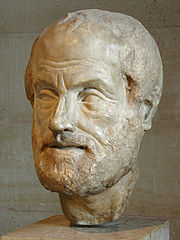
\includegraphics[scale=0.7]{Aristoteles.jpg}
    \end{column}
  \end{columns}
%\end{minipage}  
\end{frame}


\begin{frame}[t, fragile]
\frametitle{Αληθές και Ψευδές}
\begin{minipage}{\wE}
  \begin{block}{Μία ερώτηση -- Δύο απαντήσεις}
    {\bf\color{green!50!black} α) Αληθές}, \, {\bf\color{red} β) Ψευδές}
  \end{block}
  \pause
  \begin{exampleblock}{Έξω βρέχει}
     {\bf\color{green!50!black} Αληθές} \, (αν όντως βρέχει) \\
     {\bf\color{red} Ψευδές} \, (αν δεν βρέχει) \\     
  \end{exampleblock}
  \pause
  \begin{exampleblock}{Η Αθήνα είναι πρωτεύουσα της Ελλάδος}
     {\bf\color{green!50!black} Αληθές το 2012} \\
     {\bf\color{red} Ψευδές το 1830} \\     
  \end{exampleblock}
\end{minipage}  
\end{frame}



\begin{frame}[t, fragile]
\frametitle{Αληθές, Ψευδές και Άγνωστο}
\begin{minipage}{\wE}
  \begin{block}{Μία ερώτηση -- Τρεις απαντήσεις}
    {\bf\color{green!50!black} α) Αληθές}, \, {\bf\color{red} β) Ψευδές}, \, {\bf γ) Άγνωστο}
  \end{block}
  \pause
  \begin{exampleblock}{Έξω βρέχει}
     {\bf\color{green!50!black} Αληθές} \, (αν όντως βρέχει) \\
     {\bf\color{red} Ψευδές} \, (αν δεν βρέχει) \\  
     {\bf Άγνωστο} \, (δεν μπορώ να το ελέγξω) \\       
  \end{exampleblock}
  \pause
  \begin{exampleblock}{Η Αθήνα είναι πρωτεύουσα της Ελλάδος}
     {\bf\color{green!50!black} Αληθές το 2012} \\
     {\bf\color{red} Ψευδές το 1830} \\  
     {\bf Μη εφαρμόσιμο το 1730} \\       
  \end{exampleblock}
\end{minipage}  
\end{frame}


\begin{frame}[t, fragile]
\frametitle{\en Jan Łukasiewicz}
  \begin{columns}[T]
    \begin{column}{0.6\textwidth}
      %\begin{block}{ }
        \begin{enumerate}
          \item Λβιβ Γαλικίας 1878 -- Δουβλίνο 1956.
          \item Πολωνός φιλόσοφος και μαθηματικός.
          \item Πρωτεργάτης της \\ {\bf\large\color{red}  τριαδικής λογικής}.
          \item Εφευρέτης της «πολωνικής γραφής».                 
          \item Σημαντικό έργο στα μαθηματικά και την υπολογιστική επιστήμη. 
        \end{enumerate}
      %\end{block}
    \end{column}
    \begin{column}{0.4\textwidth}
      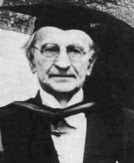
\includegraphics[scale=0.8]{Lukasiewicz.jpg}
    \end{column}
  \end{columns}
  \bigskip
\tiny Εικόνα από: {\en \url{http://en.wikipedia.org/wiki/Jan_Lukasiewicz} }  
\end{frame}


\begin{frame}[t, fragile]
\frametitle{\en Setun}
  \begin{columns}[T]
    \begin{column}{0.6\textwidth}
      %\begin{block}{ }
        \begin{enumerate}
          \item Μόσχα 1958.
          \item Ο πρώτος Η/Υ τριαδικής λογικής. 
          \item Μεγάλα πλεονεκτήματα έναντι Η/Υ δυαδικής λογικής.
          \item Το σχέδιο εγκαταλείφθηκε, λόγω μη συμμόρφωσης των στόχων με την επικρατούσα ιδεολογία.                 
          \item Άλλος ένας λόγος κατάρρευσης της Ε.Σ.Σ.Δ. 
        \end{enumerate}
      %\end{block}
    \end{column}
    \begin{column}{0.4\textwidth}
      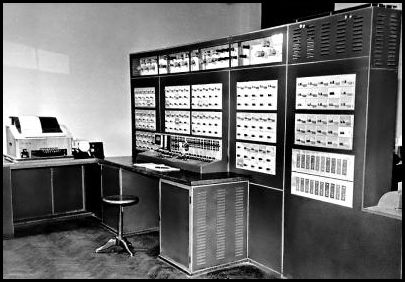
\includegraphics[scale=0.75]{setun.jpg}
    \end{column}
  \end{columns}
  \bigskip
\tiny Εικόνα από: {\en \url{http://en.wikipedia.org/wiki/Ternary_computer} }  \\
      Σχετικό άρθρο: {\en\url{http://dx.doi.org/10.1007/978-3-642-22816-2_10}}
\end{frame}



\subsection[\textlatin{Examples}] {\textgreek {Παραδείγματα} \textlatin{Null} τιμών}

\begin{frame}[t, fragile, shrink]
\frametitle{Τιμή \tnull}
\begin{minipage}{\wE}
\vspace*{-0.4cm}
  \begin{block}{Άγνωστη, μη διαθέσιμη, μη εφαρμόσιμη πληροφορία}
    Η τιμή \tnull\ αντιπροσωπεύει μια ελλιπή τιμή σε κάποιο γνώρισμα μιας σχέσης.
    Ελλιπής τιμή μπορεί να προκύψει από διάφορες αιτίες:
    \pause
    \begin{itemize}
      \item Η τιμή {\bf\color{red} υπάρχει}, αλλά είναι άγνωστη τη στιγμή της καταγραφής.
      \item Η τιμή μπορεί να {\bf\color{red} μην υπάρχει}, για μια συγκεκριμένη πλειάδα κάποιο γνώρισμα δεν έχει τιμή.
      \item Η τιμή μπορεί να {\bf\color{red} μην έχει νόημα}, για μια συγκεκριμένη πλειάδα κάποιο γνώρισμα δεν εφαρμόζεται.
    \end{itemize}
  \end{block}
  \pause
  \vspace*{-0.4cm}
  \begin{alertblock}{}%{Πολλά τα προβλήματα}
    Όσο είναι δυνατό, αποφεύγουμε την καταχώριση τιμών \tnull.
  \end{alertblock} 
\end{minipage}  
\end{frame}


\begin{frame}[t, fragile]
\frametitle{Τιμή \tnull -- Άγνωστη τιμή}
\begin{minipage}{\wE}
  \begin{tabular}{ c l l } \hline 
    {\bf Κωδικός} & {\bf Όνομα} & {\bf Αυτοκίνητο} \\ \hline  
    1025 & Βασίλης Κάππος   & ΙΧΟ 9239 \\  
    1026 & Μαρίνα Θεοδώρου  & ΙΥΓ 4561 \\  
    1027 & Νίκη Αλεξιάδου   & ΙΥΜ 5012 \\   
    1028 & Στέλιος Μακρίδης &  \\ \hline 
  \end{tabular}
  \bigskip
  \par Μια εταιρεία καταγράφει τον αριθμό κυκλοφορίας αυτοκινήτου των υπαλλήλων της έτσι ώστε
       να εισέρχονται δωρεάν στο χώρο στάθμευσης. \\ 
       Ο Στέλιος Μακρίδης είναι σε άδεια, δεν έχει ακόμη ενημερώσει για το αυτοκίνητό του την εταιρεία.
\end{minipage}  
\end{frame}


\begin{frame}[t, fragile]
\frametitle{Τιμή \tnull -- Μη διαθέσιμη τιμή}
\begin{minipage}{\wE}
  \begin{tabular}{ c l c } \hline 
    {\bf Κωδικός} & {\bf Όνομα} & {\bf Εξάμηνο} \\ \hline  
    504 & Βάσεις Δεδομένων & 5 \\  
    404 & Μακροοικονομική Θεωρία ΙΙ & 4 \\  
    303 & Προγραμματισμός Υπολογιστών Ι & 3 \\  	 
    951 & Ιστορία της Επιστημονικής Σκέψης &  \\ \hline 
  \end{tabular}
  \bigskip
  \par Το πρόγραμμα σπουδών προσφέρει ένα νέο μάθημα: «Ιστορία της Επιστημονικής Σκέψης». \\ 
       Η επιτροπή προγράμματος σπουδών δεν έχει αποφασίσει ακόμη σε ποιο εξάμηνο θα ενταχθεί το νέο μάθημα.
\end{minipage}  
\end{frame}


\begin{frame}[t, fragile]
\frametitle{Τιμή \tnull -- Μη διαθέσιμη τιμή}
\begin{minipage}{\wE}
  \begin{tabular}{ c l l } \hline 
    {\bf Κωδικός} & {\bf Όνομα} & {\bf Αυτοκίνητο} \\ \hline  
    1025 & Βασίλης Κάππος   & ΙΧΟ 9239 \\  
    1026 & Μαρίνα Θεοδώρου  & ΙΥΓ 4561 \\  
    1027 & Νίκη Αλεξιάδου   & ΙΥΜ 5012 \\  
    1028 & Στέλιος Μακρίδης &  \\ \hline 
  \end{tabular}
  \bigskip
  \par Μια εταιρεία διαθέτει αυτοκίνητο στους εξωτερικούς συνεργάτες της. \\ 
       Ο Στέλιος Μακρίδης μόλις έχει προσληφθεί, δεν του έχει ακόμα διατεθεί αυτοκίνητο.
\end{minipage}  
\end{frame}


\begin{frame}[t, fragile]
\frametitle{Τιμή \tnull -- Μη εφαρμόσιμη τιμή}
\begin{minipage}{\wE}
  \begin{tabular}{ c l c } \toprule
    {\bf Κωδικός} & {\bf Όνομα} & {\bf Εξάμηνο} \\ \midrule 
    504 & Βάσεις Δεδομένων & 5 \\ 
    404 & Μακροοικονομική Θεωρία ΙΙ & 4 \\  
    303 & Προγραμματισμός Υπολογιστών Ι & 3 \\   
    951 & Ιστορία της Επιστημονικής Σκέψης &  \\  \bottomrule
  \end{tabular}
  \bigskip
  \par Το μάθημα «Ιστορία της Επιστημονικής Σκέψης» με κωδικό 951 δεν προσφέρεται σε κάποιο
  συγκεκριμένο εξάμηνο σπουδών. \\ 
  Είναι μάθημα ελεύθερης επιλογής και οι φοιτητές
  μπορούν να το παρακολουθήσουν σε οποιοδήποτε στάδιο των σπουδών τους.
\end{minipage}  
\end{frame}



\subsection[\textlatin{NotNull}] {\textgreek {Χρήση} \textlatin{Null} τιμών και διάσπαση πινάκων}

\begin{frame}[t, fragile]
\frametitle{Πλεονεκτήματα}
\begin{minipage}{\wE}
  \begin{block}{Διάσπαση}
    Χωρίς τη δυνατότητα χρήσης των τιμών \tnull\ θα ήταν απαραίτητη {\bf\color{red} διάσπαση}
    των σχέσεων της βάσης δεδομένων σε περισσότερες ειδικές σχέσεις.
    Κάτι τέτοιο είναι βέβαια δυνατό, αλλά δυσχεραίνει τη λειτουργικότητα της βάσης δεδομένων. 
  \end{block}
  \pause
  \begin{block}{Δύο πιθανές λύσεις}
    \begin{enumerate}
      \item Διάσπαση με βάση το γνώρισμα που πιθανά παίρνει τιμές \tnull.
      \item Μεταφορά του γνωρίσματος σε νέα σχέση.
    \end{enumerate}
  \end{block}
  \par \color{blue} Περισσότερα στο κεφάλαιο της κανονικοποίησης, ακολουθούν δύο παραδείγματα.
\end{minipage}  
\end{frame}


\begin{frame}[t, fragile]
\frametitle{Διάσπαση σε δύο ειδικές σχέσεις}
\begin{minipage}{\wE} 
  \par {\color{red} Μία σχέση για μαθήματα με εξάμηνο:} \\
  \begin{tabular}{ c l c } \toprule
    {\bf Κωδικός} & {\bf Όνομα} & {\bf Εξάμηνο} \\ \midrule 
    504 & Βάσεις Δεδομένων & 5 \\ 
    404 & Μακροοικονομική Θεωρία ΙΙ & 4 \\  
    303 & Προγραμματισμός Υπολογιστών Ι & 3 \\  \bottomrule
  \end{tabular}
  \bigskip
  \par {\color{red} Και μία σχέση για μαθήματα χωρίς εξάμηνο:} \\
  \begin{tabular}{ c l } \toprule
    {\bf Κωδικός} & {\bf Όνομα}  \\ \midrule 
    951 & Ιστορία της Επιστημονικής Σκέψης \\  \bottomrule
  \end{tabular}  
\end{minipage}  
\end{frame}


\begin{frame}[t, fragile]
\frametitle{Μεταφορά γνωρίσματος σε νέα σχέση}
\begin{minipage}{\wE}
 
  \par {\color{red} Μία σχέση για τα μαθήματα:} \\
  \begin{tabular}{ c l c } \toprule
    {\bf Κωδικός} & {\bf Όνομα}  \\ \midrule 
    504 & Βάσεις Δεδομένων  \\ 
    404 & Μακροοικονομική Θεωρία ΙΙ  \\  
    303 & Προγραμματισμός Υπολογιστών Ι  \\
    951 & Ιστορία της Επιστημονικής Σκέψης \\ \bottomrule
  \end{tabular}
  \bigskip
  \par {\color{red} Και μία σχέση για το εξάμηνο των μαθημάτων:} \\
  \begin{tabular}{ c c } \toprule
    {\bf Κωδικός} & {\bf Εξάμηνο}  \\ \midrule 
    504 & 5 \\
    404 & 4 \\
    303 & 3 \\ \bottomrule
  \end{tabular}  
\end{minipage}  
\end{frame}
